% Separate exhibits file (tables and figures), as requested by IIMB Management Review
\documentclass[12pt,a4paper]{article}
% Shared preamble: IIMB Management Review submission (BAICONF 2026, BAI2575)
% Compile with pdfLaTeX + Biber (Overleaf: Menu > Compiler = pdfLaTeX; Biber runs automatically).
\usepackage[T1]{fontenc}
\usepackage[utf8]{inputenc}
\usepackage[british]{babel}
\usepackage{newtxtext,newtxmath}            % Times New Roman equivalent
\usepackage[a4paper,margin=1in]{geometry}
\usepackage{setspace}
\usepackage{amsmath,bm}
\usepackage{graphicx}
\usepackage{booktabs,tabularx,array,makecell,threeparttable}
\usepackage{pdflscape}
\usepackage[labelsep=period,font=small,labelfont=bf,justification=raggedright,singlelinecheck=false]{caption}
\captionsetup[figure]{name=Fig.}
\usepackage{xcolor}
\usepackage{microtype}
\usepackage{csquotes}
\usepackage[style=apa,backend=biber,uniquename=false]{biblatex}
\addbibresource{references.bib}
\usepackage[hidelinks]{hyperref}
\renewcommand{\cellalign}{tl}
\renewcommand{\theadalign}{tl}
\newcommand{\authorsto}[1]{\textbf{[AUTHORS TO COMPLETE: #1]}}
% Generated by R/run_all.R -- do not edit by hand
\newcommand{\nTrialsAll}{833}
\newcommand{\nAthAll}{215}
\newcommand{\nSessAll}{333}
\newcommand{\nTrials}{805}
\newcommand{\nAth}{212}
\newcommand{\nSess}{327}
\newcommand{\nTrialsS}{811}
\newcommand{\nLowcomMissing}{6}
\newcommand{\nFsLow}{60}
\newcommand{\ageMedian}{14.1}
\newcommand{\ageMin}{8.8}
\newcommand{\ageMax}{37.9}
\newcommand{\ageQone}{12.0}
\newcommand{\ageQthree}{16.8}
\newcommand{\nMinors}{164}
\newcommand{\pctMinors}{77}
\newcommand{\trialsPerAthMean}{3.8}
\newcommand{\trialsPerAthMax}{16}
\newcommand{\sessPerAthMedian}{1}
\newcommand{\sessPerAthMax}{6}
\newcommand{\trialsPerSessMedian}{2}
\newcommand{\jhMean}{28.2}
\newcommand{\jhSD}{8.4}
\newcommand{\lpfMean}{5.39}
\newcommand{\lpfSD}{1.97}
\newcommand{\lpfMin}{2.19}
\newcommand{\lpfMax}{14.88}
\newcommand{\lowcomTimeMedian}{0.24}
\newcommand{\varPCA}{37.3}
\newcommand{\varSPCA}{20.2}
\newcommand{\ldsPCA}{99.7}
\newcommand{\ldsSPCA}{96.4}
\newcommand{\peakPCA}{40}
\newcommand{\rLpfPCA}{0.39}
\newcommand{\rJhPCA}{0.13}
\newcommand{\rCtPCA}{$-$0.04}
\newcommand{\rCmdPCA}{0.01}
\newcommand{\rLdPCA}{$-$0.75}
\newcommand{\rtwoPCA}{7.7}
\newcommand{\rtwoSPCA}{19.1}
\newcommand{\cvPCA}{4.0}
\newcommand{\cvSPCA}{13.4}
\newcommand{\jhRatioPCA}{0.89}
\newcommand{\rpfRatioPCA}{1.01}
\newcommand{\jhLoPCA}{0.70}
\newcommand{\jhHiPCA}{1.06}
\newcommand{\betweenPCA}{29.6}
\newcommand{\withinPCA}{35.5}
\newcommand{\sessPCA}{34.9}
\newcommand{\betweenSPCA}{45.3}
\newcommand{\varPCB}{16.0}
\newcommand{\varSPCB}{16.6}
\newcommand{\ldsPCB}{99.9}
\newcommand{\ldsSPCB}{92.5}
\newcommand{\peakPCB}{26}
\newcommand{\rLpfPCB}{0.22}
\newcommand{\rJhPCB}{0.13}
\newcommand{\rCtPCB}{0.02}
\newcommand{\rCmdPCB}{0.00}
\newcommand{\rLdPCB}{$-$0.14}
\newcommand{\rtwoPCB}{2.7}
\newcommand{\rtwoSPCB}{5.3}
\newcommand{\cvPCB}{0.3}
\newcommand{\cvSPCB}{2.8}
\newcommand{\jhRatioPCB}{0.97}
\newcommand{\rpfRatioPCB}{1.05}
\newcommand{\jhLoPCB}{0.77}
\newcommand{\jhHiPCB}{1.16}
\newcommand{\betweenPCB}{21.4}
\newcommand{\withinPCB}{61.6}
\newcommand{\sessPCB}{17.0}
\newcommand{\betweenSPCB}{18.7}
\newcommand{\varPCC}{12.6}
\newcommand{\varSPCC}{15.1}
\newcommand{\ldsPCC}{99.5}
\newcommand{\ldsSPCC}{3.7}
\newcommand{\peakPCC}{16}
\newcommand{\rLpfPCC}{0.39}
\newcommand{\rJhPCC}{0.34}
\newcommand{\rCtPCC}{0.00}
\newcommand{\rCmdPCC}{$-$0.14}
\newcommand{\rLdPCC}{$-$0.32}
\newcommand{\rtwoPCC}{13.1}
\newcommand{\rtwoSPCC}{68.3}
\newcommand{\cvPCC}{11.8}
\newcommand{\cvSPCC}{66.4}
\newcommand{\jhRatioPCC}{0.95}
\newcommand{\rpfRatioPCC}{1.00}
\newcommand{\jhLoPCC}{0.74}
\newcommand{\jhHiPCC}{1.13}
\newcommand{\betweenPCC}{22.9}
\newcommand{\withinPCC}{74.8}
\newcommand{\sessPCC}{2.3}
\newcommand{\betweenSPCC}{26.5}
\newcommand{\varPCD}{8.9}
\newcommand{\varSPCD}{10.2}
\newcommand{\ldsPCD}{99.3}
\newcommand{\ldsSPCD}{80.2}
\newcommand{\peakPCD}{9}
\newcommand{\rLpfPCD}{0.45}
\newcommand{\rJhPCD}{0.24}
\newcommand{\rCtPCD}{0.15}
\newcommand{\rCmdPCD}{$-$0.18}
\newcommand{\rLdPCD}{$-$0.04}
\newcommand{\rtwoPCD}{9.1}
\newcommand{\rtwoSPCD}{17.8}
\newcommand{\cvPCD}{6.3}
\newcommand{\cvSPCD}{15.1}
\newcommand{\jhRatioPCD}{1.17}
\newcommand{\rpfRatioPCD}{1.05}
\newcommand{\jhLoPCD}{0.81}
\newcommand{\jhHiPCD}{1.44}
\newcommand{\betweenPCD}{10.0}
\newcommand{\withinPCD}{69.6}
\newcommand{\sessPCD}{20.3}
\newcommand{\betweenSPCD}{31.6}
\newcommand{\cumFour}{74.8}
\newcommand{\cumFourS}{62.2}
\newcommand{\cumTen}{93.8}
\newcommand{\rtwoRange}{2.7--13.1}
\newcommand{\unexplRange}{86.9--97.3}
\newcommand{\cvRange}{0.3--11.8}
\newcommand{\oneTrialRange}{4.3--17.8}
\newcommand{\athMeanRange}{5.4--21.2}
\newcommand{\adjRange}{2.0--12.4}
\newcommand{\rtwoLandingSRange}{5.3--19.1}
\newcommand{\unexplSRange}{31.7--94.7}
\newcommand{\lpfCorRange}{0.22--0.45}
\newcommand{\ctAbsMax}{0.15}
\newcommand{\cmdAbsMax}{0.18}
\newcommand{\vendorAbsMax}{0.34}
\newcommand{\rLpfSPCA}{0.71}
\newcommand{\rLdSPCA}{$-$0.57}
\newcommand{\ldsSPCCtakeoff}{96.3}
\newcommand{\rCtSPCC}{$-$0.79}
\newcommand{\rRpfSPCC}{0.77}
\newcommand{\jhBandN}{82}
\newcommand{\jhBandAth}{51}
\newcommand{\jhBandLo}{26.0}
\newcommand{\jhBandHi}{28.2}
\newcommand{\jhBandMean}{27.1}
\newcommand{\jhBandSD}{0.65}
\newcommand{\rpfBandN}{81}
\newcommand{\rpfBandAth}{58}
\newcommand{\rpfBandLo}{2.25}
\newcommand{\rpfBandHi}{2.32}
\newcommand{\jhBandSDfactor}{13}
\newcommand{\wholeJh}{1.01}
\newcommand{\wholeRpf}{1.00}
\newcommand{\wholeJhS}{1.01}
\newcommand{\rpfRatioRange}{1.00--1.05}
\newcommand{\jhRatioRange}{0.89--1.17}
\newcommand{\jhRatioOtherRange}{0.95--1.17}
\newcommand{\jhRatioSPCA}{0.82}
\newcommand{\jhLoSPCA}{0.69}
\newcommand{\jhHiSPCA}{0.96}
\newcommand{\bwPCARange}{0.87--0.89}
\newcommand{\bwAllRange}{0.84--1.17}
\newcommand{\betweenRange}{10.0--29.6}
\newcommand{\withinRange}{35.5--74.8}
\newcommand{\sessRange}{2.3--34.9}
\newcommand{\nFsLowAnalysed}{59}
\newcommand{\varShareTakeoff}{7.1}
\newcommand{\varShareLanding}{92.9}
\newcommand{\varShareTakeoffS}{31.0}
\newcommand{\rpfRatioSPCC}{0.74}
\newcommand{\rpfLoSPCC}{0.57}
\newcommand{\rpfHiSPCC}{0.87}
\newcommand{\nAthMultiSess}{83}
\newcommand{\baCIUpperRange}{23--47}
\newcommand{\baLoPCA}{13}
\newcommand{\baHiPCA}{47}
\newcommand{\baCIMaxUpper}{47}
\newcommand{\baAgeAdjRange}{7.1--28.2}
\newcommand{\baAgeMaxChange}{7.1}
\newcommand{\baAgePCA}{28.2}
\newcommand{\landRtwoPCA}{56.8}
\newcommand{\landRtwoOtherRange}{5.1--24.0}
\newcommand{\sbTrials}{3}
\newcommand{\sbPCA}{0.85}
\newcommand{\sbRange}{0.50--0.85}
\newcommand{\sdMinorPCA}{6.5}
\newcommand{\sdAdultPCA}{8.9}
\newcommand{\nTrialsMinor}{598}
\newcommand{\nZeroCmd}{1}
\newcommand{\nLowBrake}{17}
\newcommand{\nBoot}{2,000}
\newcommand{\seedValue}{2026}
\newcommand{\nRepro}{42}
\newcommand{\nReproTotal}{42}

% Figure captions (greyscale figures; numbers come from numbers.tex)
\newcommand{\capMean}{(A) Mean body-weight-normalised vertical force (line) $\pm$ 1 SD (shaded) of the \nTrials{} analysed countermovement jumps. The take-off phase (movement onset to take-off) and the landing phase (touch-down to the lowest point of the centre of mass, COM) were each time-normalised to 0--100\% and concatenated; flight is omitted. The dotted line marks body weight. (B) Variance explained by each of the first ten principal components (bars) and cumulatively (line); the dashed line marks the four retained components.}
\newcommand{\capPCs}{Interpretation of the four retained principal components (main analysis). Each panel shows the mean curve (thin grey line) and the mean curve plus (solid black line) or minus (dashed black line) two standard deviations of the component score. Values below zero in the reconstructions are an artefact of adding a linear component to the mean and do not correspond to observed trials. The vertical line separates the take-off and landing phases.}
\newcommand{\capBand}{Trials matched on jump height do not share a common force--time curve. (A) Curves of the \jhBandN{} trials between the 45th and 55th percentiles of jump height (\jhBandMean{} $\pm$ \jhBandSD{}\,cm), shaded from light grey (low) to black (high) by their PC1 score. (B) Ratio of the standard deviation of each component score among trials matched on jump height (black circles) or on relative concentric peak force (grey triangles) to that in the full sample, with athlete-level bootstrap 95\% confidence intervals. A ratio of 1 indicates that matching on the metric leaves curve-shape variation unchanged.}
\newcommand{\capRtwo}{Proportion of the variance of each component score explained by the four vendor metrics, age and body mass, under four evaluation schemes (bars from black to white: in-sample, athlete-grouped cross-validation, one trial per athlete, athlete means), for the main landing definition (left) and the 1-s landing window (right). CV, cross-validation with athletes allocated to folds.}
\newcommand{\capWindow}{Sensitivity analysis with the landing phase ending 1\,s after touch-down: mean curve (thin grey line) and the mean curve plus (solid black line) or minus (dashed black line) two standard deviations of each retained component. Under this definition PC3 is located almost entirely in the take-off phase (\ldsSPCCtakeoff\% of its squared loading) and describes the duration and amplitude of the propulsive force.}

\graphicspath{{figures/}}
\setlength{\emergencystretch}{2em}
% Testing period: min--max recorded date (IST) of the 327 analysed sessions in the raw export (derived 13 Nov 2026)
\newcommand{\testPeriod}{November 2022 and April 2026}
% Title, short title, abstract, keywords and extended summary (anonymised; IIMB MR page 2 requirements)
\newcommand{\papertitle}{Revealing hidden jump strategies beyond conventional force-plate metrics}
\newcommand{\shorttitle}{Hidden strategies in jump curves}


\begin{document}
\begin{center}{\large\bfseries Exhibits (tables and figures) for: \papertitle\par}\end{center}
\section*{Tables}
% Generated from package/output/paper_tables_latex/tab1_qc.tex (R pipeline); only layout changed.
\begin{table}[tbp]
\centering
\begin{threeparttable}
\caption{Quality-control flow (main analysis).}
\label{tab:qc}
\small
\begin{tabular*}{\linewidth}{@{\extracolsep{\fill}}lrrr@{}}
\toprule
Step & Trials & Sessions & Athletes \\
\midrule
All male football CMJ trials & 833 & 333 & 215 \\
R1: valid body mass & 828 & 329 & 212 \\
R2: quiet-stance mass within 5\% of body mass & 813 & 328 & 212 \\
R3: no force on plate during flight & 811 & 327 & 212 \\
R4: complete metrics and age & 811 & 327 & 212 \\
R5: end of landing (lowest COM) found & 805 & 327 & 212 \\
\bottomrule
\end{tabular*}
\begin{tablenotes}[flushleft]\footnotesize
\item \textit{Note.} Rules R1--R4 were fixed before any result was examined; R5 applies only to the main landing definition (touch-down to the lowest point of the centre of mass), and the 1-s landing window therefore retained \nTrialsS{} trials. Sessions are test occasions on which an athlete performed one or more trials. COM = centre of mass.
\end{tablenotes}
\end{threeparttable}
\end{table}
\clearpage
% Generated from package/output/paper_tables_latex/tab2_descriptives.tex (R pipeline); only layout changed.
\begin{table}[tbp]
\centering
\begin{threeparttable}
\caption{Characteristics of the analysed sample (\nTrials{} trials, \nAth{} athletes).}
\label{tab:desc}
\footnotesize
\setlength{\tabcolsep}{3pt}
\begin{tabular*}{\linewidth}{@{\extracolsep{\fill}}>{\raggedright\arraybackslash}p{0.30\linewidth}rlll@{}}
\toprule
Variable & $n$ & Mean $\pm$ SD & Median (IQR) & Range \\
\midrule
Age at first test (years) & 212 & 16.01 $\pm$ 5.94 & 14.10 (12.00--16.80) & 8.80--37.90 \\
Body mass at first test (kg) & 212 & 53.31 $\pm$ 15.90 & 51.73 (40.86--64.03) & 25.03--95.97 \\
Jump height, flight time (cm) & 805 & 28.19 $\pm$ 8.43 & 26.96 (21.62--34.69) & 8.54--51.47 \\
Concentric peak force (N) & 805 & 1269.26 $\pm$ 420.74 & 1227.01 (923.47--1582.99) & 473.52--3073.22 \\
Concentric peak force ($\times$\,BW) & 805 & 2.35 $\pm$ 0.38 & 2.29 (2.11--2.51) & 1.65--4.70 \\
Eccentric braking impulse (N\,s) & 805 & 27.80 $\pm$ 15.43 & 24.60 (16.59--35.70) & 0.00--95.18 \\
Concentric impulse, first 100 ms (N\,s) & 805 & 62.24 $\pm$ 26.66 & 58.70 (41.76--79.14) & 1.51--187.93 \\
Peak landing force ($\times$\,BW) & 805 & 5.39 $\pm$ 1.97 & 4.97 (3.88--6.67) & 2.19--14.88 \\
Contraction time (s) & 805 & 0.78 $\pm$ 0.19 & 0.77 (0.66--0.90) & 0.31--1.48 \\
Countermovement depth (cm) & 805 & $-$26.55 $\pm$ 9.90 & $-$27.13 ($-$33.55--$-$20.71) & $-$52.39--0.00 \\
Touch-down--lowest COM (s) & 805 & 0.25 $\pm$ 0.11 & 0.24 (0.15--0.31) & 0.07--0.93 \\
Trials per athlete & 212 & 3.80 $\pm$ 2.28 & 3.00 (2.00--5.00) & 1.00--16.00 \\
Trials per session & 327 & 2.46 $\pm$ 0.78 & 2.00 (2.00--3.00) & 1.00--7.00 \\
Sessions per athlete & 212 & 1.54 $\pm$ 0.80 & 1.00 (1.00--2.00) & 1.00--6.00 \\
\bottomrule
\end{tabular*}
\begin{tablenotes}[flushleft]\footnotesize
\item \textit{Note.} Age and body mass are per athlete at the first analysed trial; all other rows are per trial unless stated. Jump height is derived from flight time. Countermovement depth is the vendor estimate of centre-of-mass displacement (negative downwards). Touch-down to lowest COM is the duration of the landing phase in the main analysis. BW = body weight; COM = centre of mass; IQR = interquartile range.
\end{tablenotes}
\end{threeparttable}
\end{table}
\clearpage
% Generated by build2/mktab.py from the R pipeline output (tab3_components.tex); layout only.
\begin{table}[!htbp]
\centering
\begin{threeparttable}
\caption{Retained principal components (main analysis)}
\label{tab:pcs}
\footnotesize\setlength{\tabcolsep}{4pt}
\begin{tabular}{@{}l S[table-format=2.1] S[table-format=2.1] S[table-format=2.1] S[table-format=2.0] *{5}{S[table-format=-1.2]}@{}}
\toprule
 & {Variance} & {Cumulative} & {Landing} & {Peak} & \multicolumn{5}{c}{Pearson $r$ with} \\
\cmidrule(l){6-10}
Component & {(\%)} & {(\%)} & {share (\%)} & {at (\%)} & {LPF} & {JH} & {CT} & {CMD} & {LD} \\
\midrule
PC1 & 37.3 & 37.3 & 99.7 & 40 & 0.39 & 0.13 & -0.04 & 0.01 & -0.75 \\
PC2 & 16.0 & 53.3 & 99.9 & 26 & 0.22 & 0.13 & 0.02 & 0.00 & -0.14 \\
PC3 & 12.6 & 65.9 & 99.5 & 16 & 0.39 & 0.34 & 0.00 & -0.14 & -0.32 \\
PC4 & 8.9 & 74.8 & 99.3 & 9 & 0.45 & 0.24 & 0.15 & -0.18 & -0.04 \\
\bottomrule
\end{tabular}
\begin{tablenotes}[flushleft]\footnotesize
\item \textit{Note.} Landing share = percentage of the squared loading vector that lies in the landing block (the rest is in take-off). Peak at = position of the largest absolute loading, in \% of the landing phase. Signs are set so that the largest absolute loading is positive. LPF = peak landing force relative to body weight; JH = jump height; CT = contraction time; CMD = countermovement depth; LD = landing duration (touch-down to lowest COM).
\end{tablenotes}
\end{threeparttable}
\end{table}
\clearpage
% Generated by build2/mktab.py from the R pipeline output (tab4_bands.tex); layout only.
\begin{table}[!htbp]
\centering
\begin{threeparttable}
\caption{Score dispersion among trials matched on jump height or relative peak force}
\label{tab:band}
\footnotesize\setlength{\tabcolsep}{4pt}
\begin{tabular}{@{}l S[table-format=2.2] S[table-format=2.2] S[table-format=1.2] c S[table-format=2.2] S[table-format=1.2] c@{}}
\toprule
 & {Full sample} & \multicolumn{3}{c}{Jump-height band} & \multicolumn{3}{c}{Relative peak-force band} \\
\cmidrule(lr){3-5}\cmidrule(l){6-8}
Component & {SD} & {SD} & {Ratio} & 95\% CI & {SD} & {Ratio} & 95\% CI \\
\midrule
PC1 & 7.28 & 6.45 & 0.89 & {[0.70, 1.06]} & 7.33 & 1.01 & {[0.77, 1.16]} \\
PC2 & 4.77 & 4.62 & 0.97 & {[0.77, 1.16]} & 5.01 & 1.05 & {[0.82, 1.24]} \\
PC3 & 4.22 & 4.03 & 0.95 & {[0.74, 1.13]} & 4.25 & 1.00 & {[0.81, 1.17]} \\
PC4 & 3.56 & 4.16 & 1.17 & {[0.81, 1.44]} & 3.75 & 1.05 & {[0.87, 1.23]} \\
\addlinespace
Whole curve$^{a}$ & 11.92 & 11.99 & 1.01 & {} & 11.95 & 1.00 & {} \\
\bottomrule
\end{tabular}
\begin{tablenotes}[flushleft]\footnotesize
\item \textit{Note.} Bands contain the trials between the 45th and 55th percentiles of jump height (\jhBandLo--\jhBandHi\,cm; \jhBandN{} trials, \jhBandAth{} athletes) or of concentric peak force relative to body weight (\rpfBandLo--\rpfBandHi\,BW; \rpfBandN{} trials, \rpfBandAth{} athletes). Ratio = SD in the band divided by SD in the full sample; a ratio of 1 means that matching left the spread unchanged. CIs are percentile intervals from \nBoot{} athlete-level bootstrap resamples, conditional on the estimated components. Component SDs are in score units and are comparable only within this table. $^{a}$Square root of the summed point-wise variance of the 202-point curve.
\end{tablenotes}
\end{threeparttable}
\end{table}
\clearpage
% Generated from package/output/paper_tables_latex/tab5_r2.tex (R pipeline); only layout changed.
\begin{table}[tbp]
\centering
\begin{threeparttable}
\caption{Variance of each component score explained by the four vendor metrics, age and body mass, and decomposition of component-score variance (main analysis).}
\label{tab:r2}
\footnotesize
\setlength{\tabcolsep}{2.5pt}
\begin{tabular*}{\linewidth}{@{\extracolsep{\fill}}lrrrrrrrr@{}}
\toprule
 & \multicolumn{5}{c}{$R^2$ on metrics, age and body mass (\%)} & \multicolumn{3}{c}{Variance of score (\%)} \\
\cmidrule(lr){2-6}\cmidrule(l){7-9}
Component & \makecell[r]{In-\\sample} & Adjusted & \makecell[r]{Athlete\\CV} & \makecell[r]{One trial\\per athlete} & \makecell[r]{Athlete\\means} & \makecell[r]{Between\\athletes} & \makecell[r]{Between\\sessions} & \makecell[r]{Within\\session} \\
\midrule
PC1 & 7.7 & 7.0 & 4.0 & 10.0 & 11.1 & 29.6 & 34.9 & 35.5 \\
PC2 & 2.7 & 2.0 & 0.3 & 4.3 & 5.4 & 21.4 & 17.0 & 61.6 \\
PC3 & 13.1 & 12.4 & 11.8 & 17.8 & 21.2 & 22.9 & 2.3 & 74.8 \\
PC4 & 9.1 & 8.4 & 6.3 & 11.1 & 13.8 & 10.0 & 20.3 & 69.6 \\
\bottomrule
\end{tabular*}
\begin{tablenotes}[flushleft]\footnotesize
\item \textit{Note.} Predictors: jump height, concentric peak force, eccentric braking impulse, concentric impulse over the first 100\,ms, age and body mass (ordinary least squares). In-sample and adjusted values use all \nTrials{} trials. Athlete CV = out-of-sample $R^2$ from five-fold cross-validation with athletes, not trials, allocated to folds. One trial per athlete = one randomly drawn trial per athlete (\nAth{} trials). Athlete means = scores and predictors averaged within athlete. Variance shares come from a three-level random-intercept model (athlete, session within athlete, trial within session) fitted by restricted maximum likelihood.
\end{tablenotes}
\end{threeparttable}
\end{table}
\clearpage
% Generated from package/output/paper_tables_latex/tab6_variance.tex (R pipeline); only layout changed.
\begin{table}[H]
\centering
\begin{threeparttable}
\caption{Decomposition of component-score variance between athletes, sessions and trials (main analysis, \% of total variance).}
\label{tab:vd}
\small
\begin{tabular*}{\linewidth}{@{\extracolsep{\fill}}lllll@{}}
\toprule
Component & \makecell[l]{Between\\athletes} & \makecell[l]{Between\\sessions} & \makecell[l]{Within\\session} & \makecell[l]{Between athletes,\\age-adjusted} \\
\midrule
PC1 & 29.6 (13--47) & 34.9 (16--53) & 35.5 (26--46) & 28.2 \\
PC2 & 21.4 (4--37) & 17.0 (3--36) & 61.6 (50--73) & 20.6 \\
PC3 & 22.9 (12--31) & 2.3 (0--14) & 74.8 (63--85) & 15.9 \\
PC4 & 10.0 (0--23) & 20.3 (9--32) & 69.6 (59--79) & 7.1 \\
\bottomrule
\end{tabular*}
\begin{tablenotes}[flushleft]\footnotesize
\item \textit{Note.} Three-level random-intercept model (athlete, session within athlete, trial within session) fitted by restricted maximum likelihood. Values in parentheses are 95\% CIs from \nBoot{} athlete-level bootstrap resamples. Only \nAthMultiSess{} of the \nAth{} athletes contributed more than one session, so the between-session share is imprecise. Age-adjusted = the same model with age at test as a fixed effect.
\end{tablenotes}
\end{threeparttable}
\end{table}
\clearpage
% Generated by build2/mktab.py from the R pipeline output (tab7_windows.tex); layout only.
\begin{table}[!htbp]
\centering
\begin{threeparttable}
\caption{Main analysis compared with the 1-s landing window}
\label{tab:window}
\footnotesize\setlength{\tabcolsep}{3.5pt}
\begin{tabular}{@{}l *{8}{S[table-format=2.1, table-column-width=2.2em]}@{}}
\toprule
 & \multicolumn{4}{c}{Main analysis$^{a}$} & \multicolumn{4}{c}{1-s landing window} \\
\cmidrule(lr){2-5}\cmidrule(l){6-9}
 & {PC1} & {PC2} & {PC3} & {PC4} & {PC1} & {PC2} & {PC3} & {PC4} \\
\midrule
\multicolumn{9}{@{}l}{\textit{Panel A. By component}} \\
\quad Variance explained (\%) & 37.3 & 16.0 & 12.6 & 8.9 & 20.2 & 16.6 & 15.1 & 10.2 \\
\quad Landing share of loading (\%) & 99.7 & 99.9 & 99.5 & 99.3 & 96.4 & 92.5 & 3.7 & 80.2 \\
\quad In-sample $R^2$ (\%) & 7.7 & 2.7 & 13.1 & 9.1 & 19.1 & 5.3 & 68.3 & 17.8 \\
\quad Athlete-CV $R^2$ (\%) & 4.0 & 0.3 & 11.8 & 6.3 & 13.4 & 2.8 & 66.4 & 15.1 \\
\quad Between-athlete variance (\%) & 29.6 & 21.4 & 22.9 & 10.0 & 45.3 & 18.7 & 26.5 & 31.6 \\
\addlinespace
\multicolumn{9}{@{}l}{\textit{Panel B. Summary measures}} \\
\quad Trials / athletes after quality control & \multicolumn{4}{c}{805 / 212} & \multicolumn{4}{c}{811 / 212} \\
\quad Cumulative variance, PC1--PC4 (\%) & \multicolumn{4}{c}{74.8} & \multicolumn{4}{c}{62.2} \\
\quad PC1 SD ratio, jump-height band [95\% CI] & \multicolumn{4}{c}{0.89 [0.70, 1.06]} & \multicolumn{4}{c}{0.82 [0.69, 0.96]} \\
\quad PC3 SD ratio, relative-peak-force band [95\% CI] & \multicolumn{4}{c}{1.00 [0.81, 1.17]} & \multicolumn{4}{c}{0.74 [0.57, 0.87]} \\
\quad Whole-curve SD ratio, jump-height band & \multicolumn{4}{c}{1.01} & \multicolumn{4}{c}{1.01} \\
\quad $r$(PC1, peak landing force) & \multicolumn{4}{c}{0.39} & \multicolumn{4}{c}{0.71} \\
\quad $r$(PC3, contraction time) & \multicolumn{4}{c}{0.00} & \multicolumn{4}{c}{$-$0.79} \\
\bottomrule
\end{tabular}
\begin{tablenotes}[flushleft]\footnotesize
\item \textit{Note.} $^{a}$Landing from touch-down to the lowest COM point. Between-athlete variance is from the three-level random-intercept model (Table~\ref{tab:vd}). Under the 1-s window PC3 is a take-off component (Fig.~\ref{fig:window}), which explains its correlation with contraction time and its narrower spread among trials matched on relative peak force. CI = confidence interval; COM = centre of mass; CV = cross-validation; QC = quality control.
\end{tablenotes}
\end{threeparttable}
\end{table}
\clearpage
\section*{Figures}
\begin{figure}[p]\centering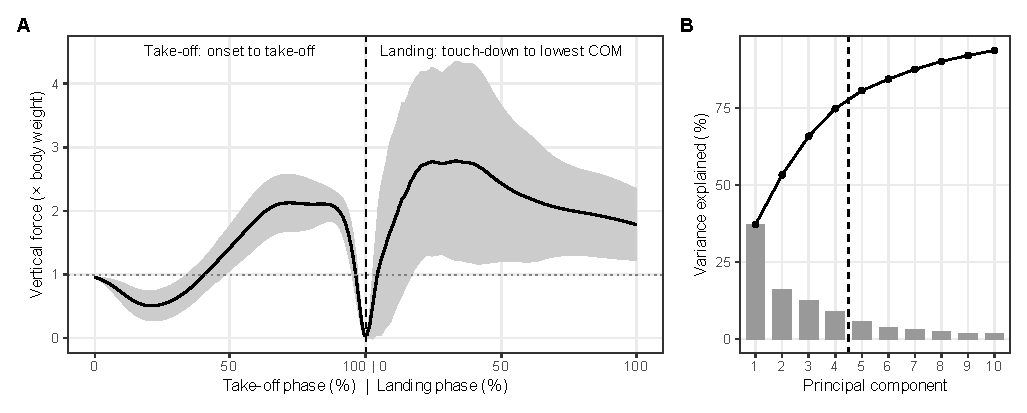
\includegraphics[width=\linewidth]{Fig1_mean_curve_scree}\caption{\capMean}\label{fig:mean}\end{figure}\clearpage
\begin{figure}[p]\centering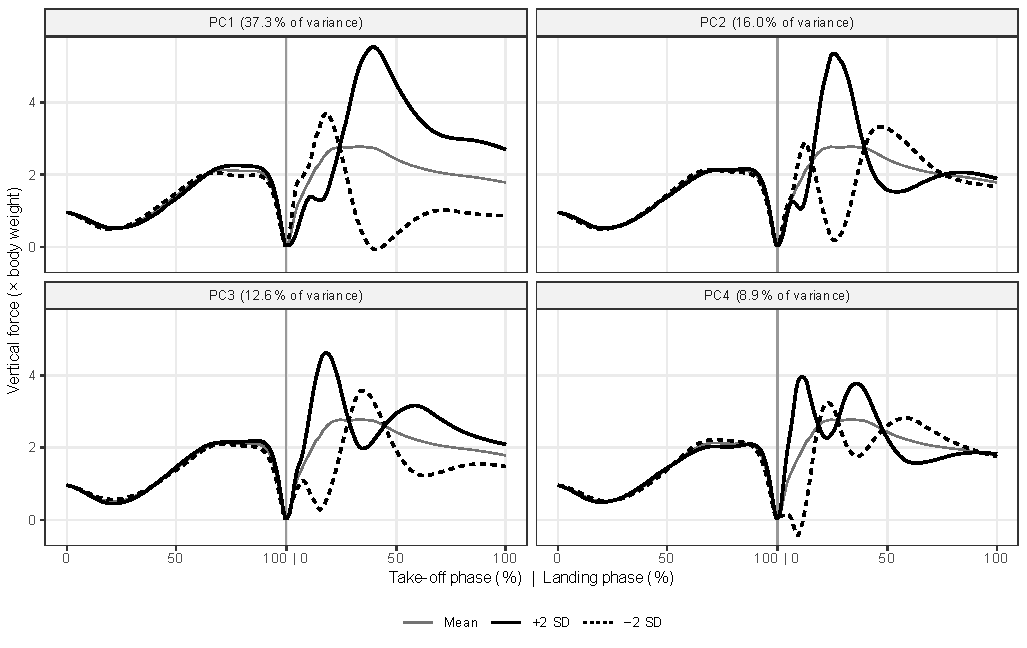
\includegraphics[width=\linewidth]{Fig2_pc_reconstructions_main}\caption{\capPCs}\label{fig:pcs}\end{figure}\clearpage
\begin{figure}[p]\centering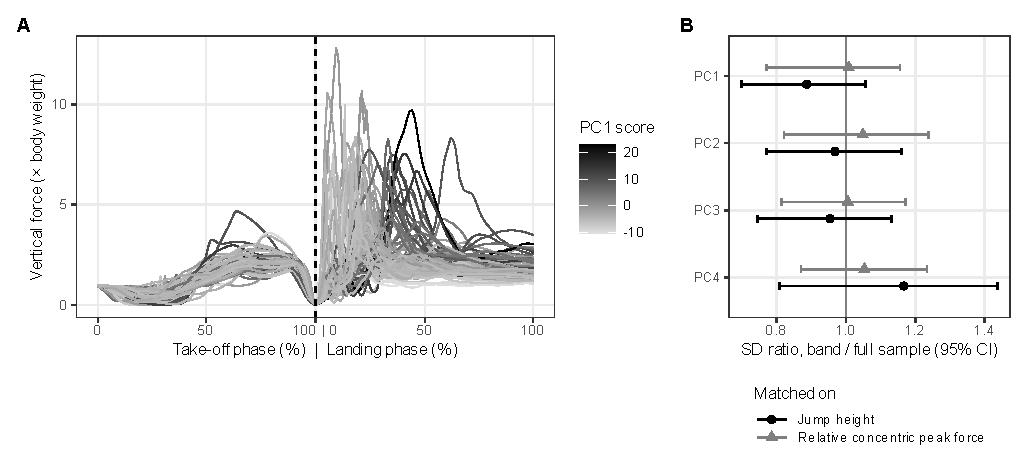
\includegraphics[width=\linewidth]{Fig3_matched_band}\caption{\capBand}\label{fig:band}\end{figure}\clearpage
\begin{figure}[p]\centering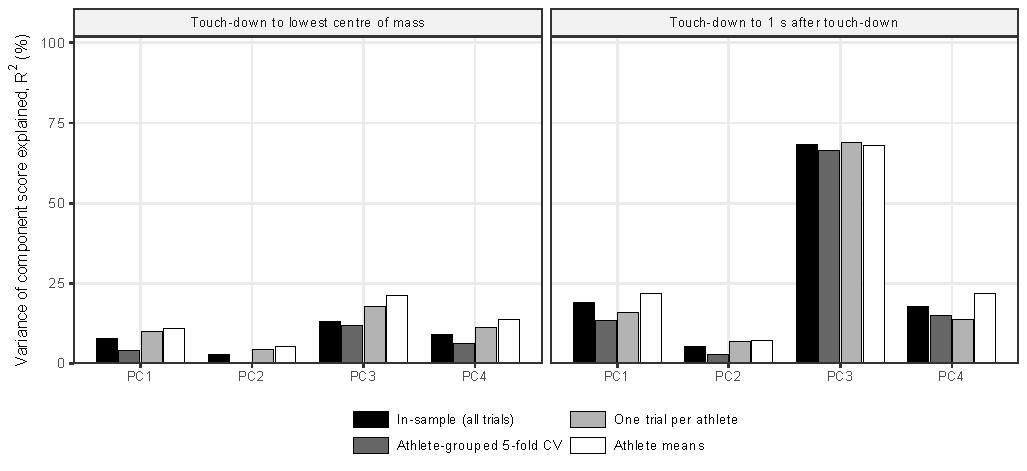
\includegraphics[width=\linewidth]{Fig4_variance_explained}\caption{\capRtwo}\label{fig:r2}\end{figure}\clearpage
\begin{figure}[p]\centering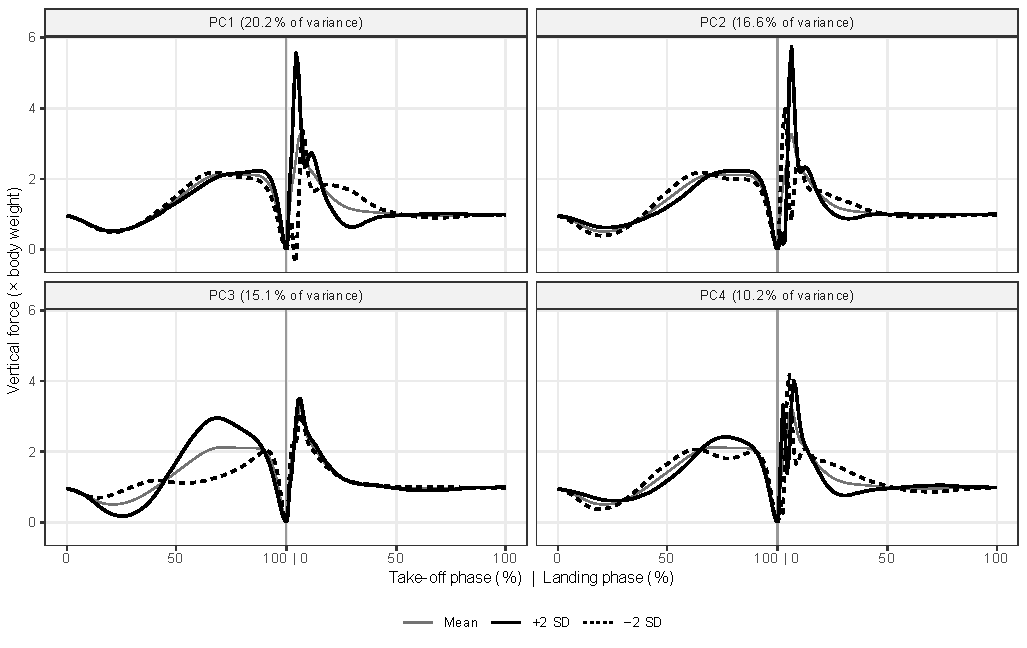
\includegraphics[width=\linewidth]{Fig5_pc_reconstructions_1s}\caption{\capWindow}\label{fig:window}\end{figure}
\end{document}
